\clearpage
\section{Hamming Encoder/Decoder Chain}

\begin{refsection}

\begin{tcolorbox}	
	\begin{tabular}{p{2.75cm} p{0.2cm} p{10.5cm}} 	
		\textbf{Students Name} &:& Lu\'{i}s Almeida (08/06/2018 - ?) \\
		\textbf{Goal}          &:& Hamming Channel Encoder/Decoder implementation.
	\end{tabular}
\end{tcolorbox}

Hamming Channel Encoder/Decoder simulates a channel encoder and decoder that uses the Hamming Algorithm. The goal is to perform the encoding of supplied source data, then encode it using the Hamming Encoder, pass the encoded data through a channel that implements errors according to a defined probability and finally perform the decoding using the Hamming Decoder. In the end a BER is performed to detect the possibility of errors.

\subsection{Introduction}
\begin{tcolorbox}	
	\begin{tabular}{p{2.75cm} p{0.2cm} p{10.5cm}} 	
		\textbf{Students Name} &:& Lu\'{i}s Almeida (08/06/2018 - ?)\\
		\textbf{Goal}          &:& Hamming Channel Encoder/Decoder protocol description.
	\end{tabular}
\end{tcolorbox}

The Hamming code is a linear block code, was developed by Richard Hamming, is used in signal processing and telecommunications. Its use allows the transfer and storage of data in a safe and efficient way.

In telecommunications the Hamming codes used are generalizations of Hamming Code (7,4). These can detect errors up to two bits and correct up to one bit. In contrast, the parity code cannot fix errors, and can only detect an odd number of errors. Due to its simplicity the Hamming codes are widely used in computer memory (ECC). In this context, it is common to use an extended Hamming code with an extra parity bit.

In mathematical terms, Hamming codes are a class of binary linear codes. For each integer $r \geq 2$ there is a block length $n = 2^{r} -1$ and message length $k = 2^{r} - r - 1$. Therefore, the Hamming code rate is $R = k / n = 1 - r / (2^{r}r - 1)$, which is as high as possible for codes with distance $3$ and block length $2^{r} - 1$. The parity matrix of a Hamming code is constructed by listing all columns of length $r$ that are linearly independent. Hamming codes are special because they are perfect codes, that is, they reach the highest rate for the codes with their block length and a minimum distance of $3$ \cite{venkatesanguruswami2010}.

\subsection{Theoretical Analysis}

One of the most used Hamming Codes is the (7, 4), that encodes 4 data bits into 7 bit block (3 extra parity bits). The extra 3 bits will enable the receiver to detect up to 2 errors and correct one of them.

In order to encode a block of 4 data bits it is required to have a generator matrix $G$. Multiplying $[d1 ~ d2 ~ d3 ~ d4] \times G(d)]$ will result in the desired $1 \times 7$ encoded word.

The $G$ matrix can be defined for the Hamming Code $(7, 4)$ as follows:

\begin{equation}
G = [p | d];
\end{equation}

where,

\begin{equation}
	p = \begin{bmatrix}
	0 & 1 & 1 \\ 
	1 & 0 & 1 \\ 
	1 & 1 & 0 \\ 
	1 & 1 & 1 
	\end{bmatrix}
\end{equation}

\begin{equation}
	d = \begin{bmatrix}
	1 & 0 & 0 & 0 \\ 
	0 & 1 & 0 & 0 \\ 
	0 & 0 & 1 & 0 \\ 
	0 & 0 & 0 & 1
	\end{bmatrix}
\end{equation}

Also for decode it is required to create a decoding matrix $H$, and using the same example Hamming Code $(7, 4)$, we can form the $H$ matrix as follows.

\begin{equation}
H = \begin{bmatrix}
1 & 0 & 0 & 0 & 1 & 1 & 1 \\ 
0 & 1 & 0 & 1 & 0 & 1 & 1 \\ 
0 & 0 & 1 & 1 & 1 & 0 & 1
\end{bmatrix}
\end{equation}

Using the $H$ matrix we can detect the presence of errors in the received 7 bit block. If we multiply $H$ by the 7 bit block the outcome will be a $3 \times 1$ vector $(err)$ that if the sum of it's values is different than zero it means an error was detected.

So to correct that error, we just need to compare the $(err)$ with the $H$ matrix and search for the column that is equal to the obtained $err$ vector. That indicates the bit that was received wrongly. To correct it, we just need to change the corresponding bit value.

After that to perform the decoding we just need to segment the last 4 bits from the 7 bit vector in order to recover the 4 data bits sent.

\subsection{Simulation Analysis}

The project flow can be observed in Figure \ref{fig:hammingEncoderDecoder}.

\begin{figure}[h!]
	\vspace{-3mm}
	\centering
	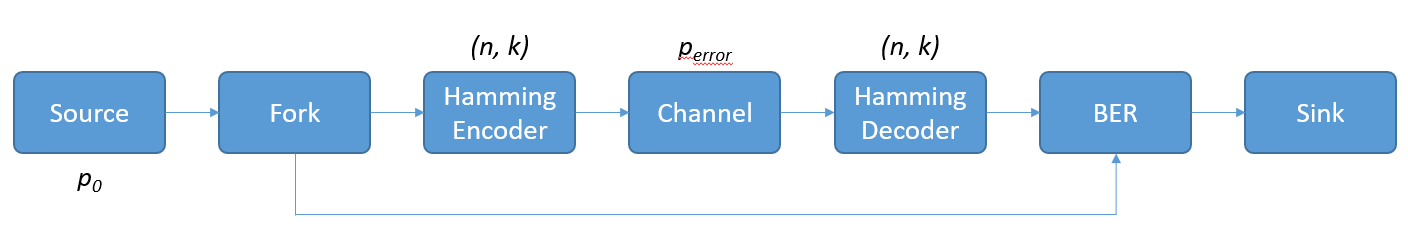
\includegraphics[width=.9\linewidth]{./sdf/eit_25828_hamming_channel_encoder_decoder/images/blockDesign.png}
	\vspace{-3mm}
	\caption{Hamming Encoder/Decoder Design Flow}
	\label{fig:hammingEncoderDecoder}
	\vspace{-3mm}
\end{figure}

Initially the project uses a Binary Source block in order to create a random number of bits that form the Data Signal $S0$ (Figure \ref{fig:hammingEncoderDecoder_S0}).

\begin{figure}[h!]
	\centering
	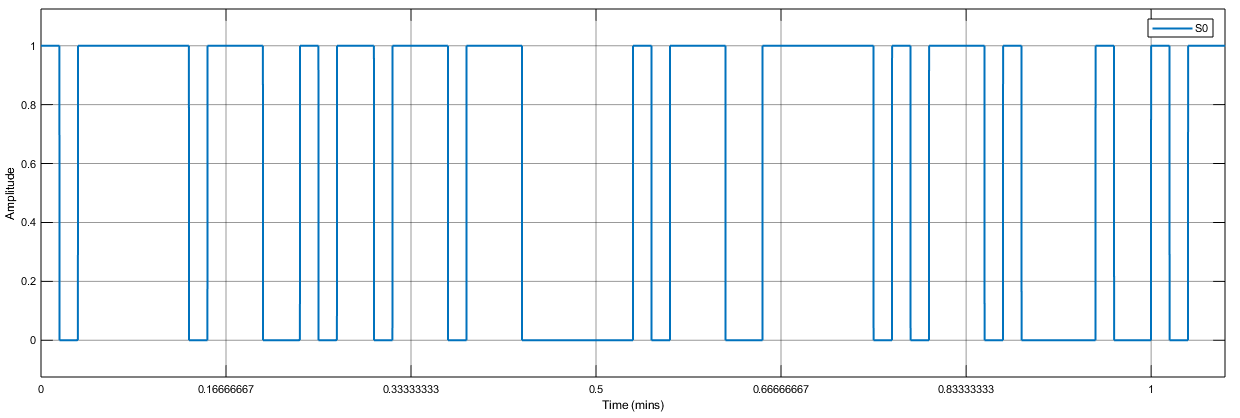
\includegraphics[width=.9\linewidth]{./sdf/eit_25828_hamming_channel_encoder_decoder/images/S0.png}
	\vspace{-3mm}
	\caption{S0 Signal Example for Hamming Code (7, 4)}
	\label{fig:hammingEncoderDecoder_S0}
\end{figure}

Next the $S0$ is feed into a Fork block in order to create a copy of the original signal, $S0$, so it can be feed into the following processing chain and into the BER block.

After that $S0$ is encoded using the Hamming Encoder Block and we obtain the encoded signal $S1$, according to the selected Hamming Code $(n, k)$ (Figure \ref{fig:hammingEncoderDecoder_S1}).

\begin{figure}[h!]
	\centering
	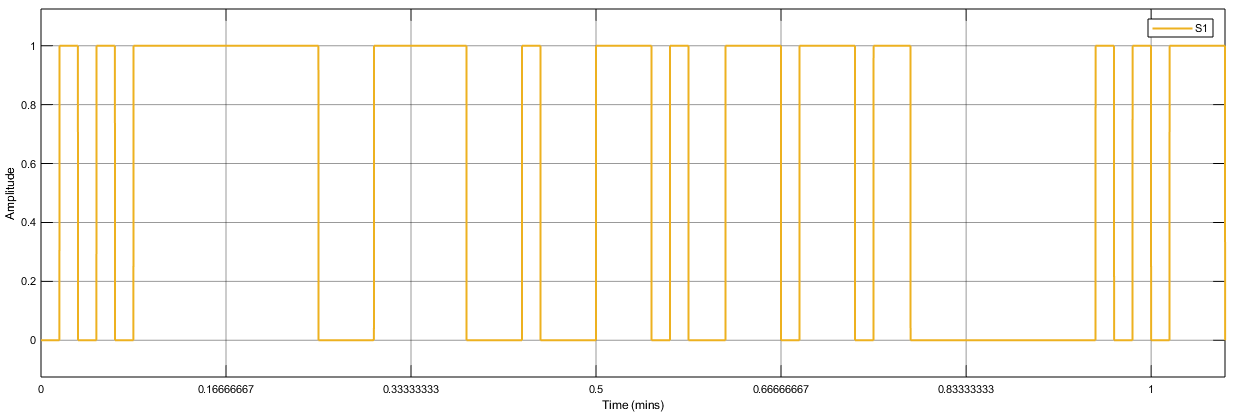
\includegraphics[width=.9\linewidth]{./sdf/eit_25828_hamming_channel_encoder_decoder/images/S1.png}
	\vspace{-3mm}
	\caption{S1 Signal Example for Hamming Code (7, 4)}
	\label{fig:hammingEncoderDecoder_S1}
\end{figure}

In order to simulate the occurrence of errors a second Binary Source block is used to generate the noise signal, $S2$, that basically produces a one accordingly to a given percentage, where it represents an error (Figure \ref{fig:hammingEncoderDecoder_S2}).

\begin{figure}[h!]
	\centering
	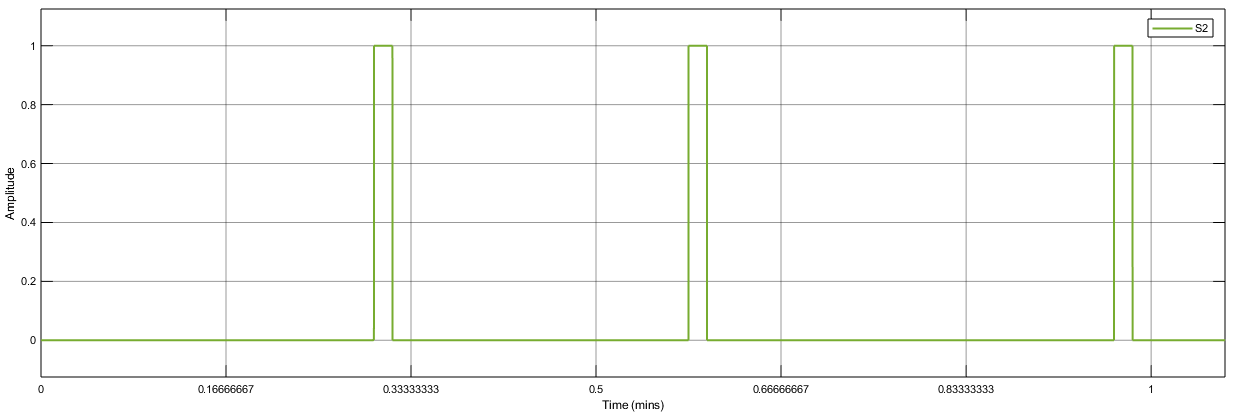
\includegraphics[width=.9\linewidth]{./sdf/eit_25828_hamming_channel_encoder_decoder/images/S2.png}
	\vspace{-3mm}
	\caption{S2 Signal Example for Hamming Code (7, 4)}
	\label{fig:hammingEncoderDecoder_S2}
\end{figure}

\vspace{60mm}

After that the data signal, $S0$, is summed, using an add block, with the noise signal, $S2$, and we obtain the data signal with errors, $S3$, simulating a noise channel (Figure \ref{fig:hammingEncoderDecoder_S3} and Figure \ref{fig:hammingEncoderDecoder_S1_S3}).

\begin{figure}[h!]
	\centering
	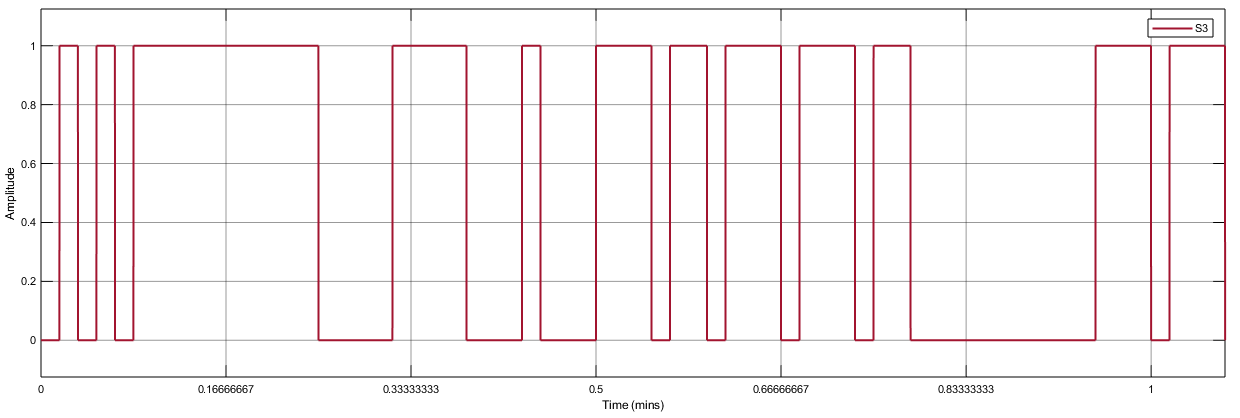
\includegraphics[width=.9\linewidth]{./sdf/eit_25828_hamming_channel_encoder_decoder/images/S3.png}
	\vspace{-3mm}
	\caption{S3 Signal Example for Hamming Code (7, 4)}
	\label{fig:hammingEncoderDecoder_S3}
\end{figure}

\begin{figure}[h!]
	\centering
	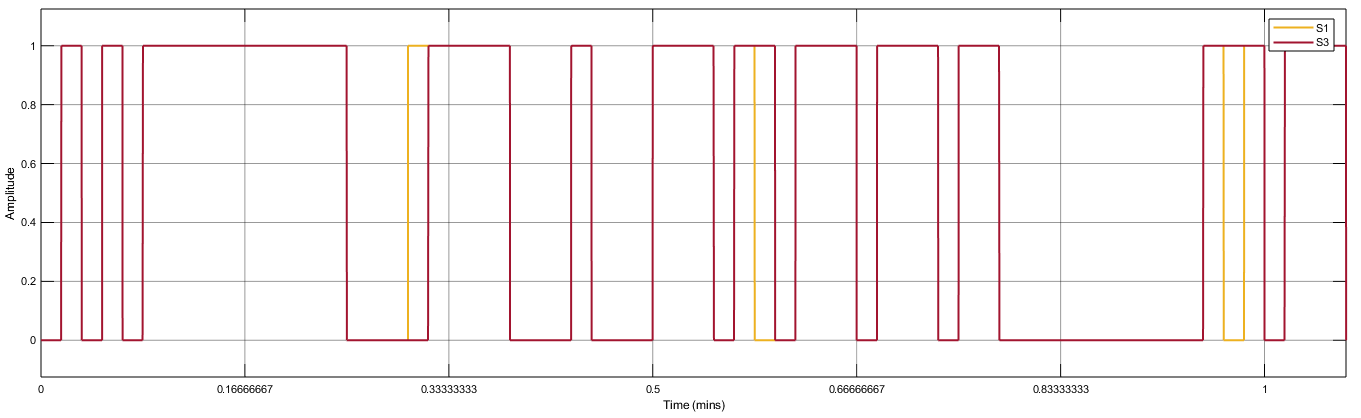
\includegraphics[width=.9\linewidth]{./sdf/eit_25828_hamming_channel_encoder_decoder/images/S1_S3.png}
	\vspace{-3mm}
	\caption{Comparison of S1 and S3 Signals}
	\label{fig:hammingEncoderDecoder_S1_S3}
\end{figure}

Then the obtained signal is decoded using the Hamming Decoder block, returning the decoded signal, $S4$ (Figure \ref{fig:hammingEncoderDecoder_S4}).

\begin{figure}[h!]
	\centering
	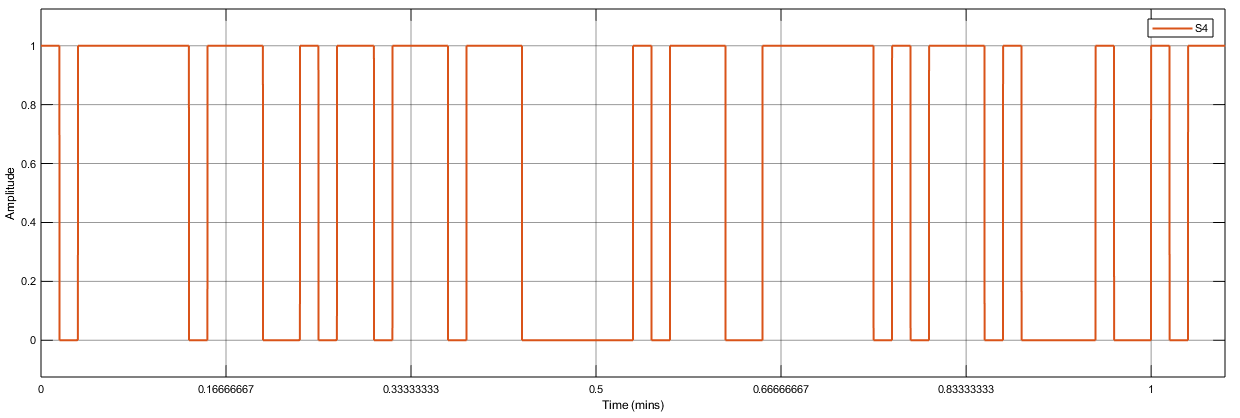
\includegraphics[width=.9\linewidth]{./sdf/eit_25828_hamming_channel_encoder_decoder/images/S4.png}
	\vspace{-3mm}
	\caption{S4 Signal Example for Hamming Code (7, 4)}
	\label{fig:hammingEncoderDecoder_S4}
\end{figure}

Finally a BER comparison using the BER block is performed in order to evaluate the encoding and decoding chain (Figure \ref{fig:hammingEncoderDecoder_S0_S4}).

\begin{figure}[h!]
	\centering
	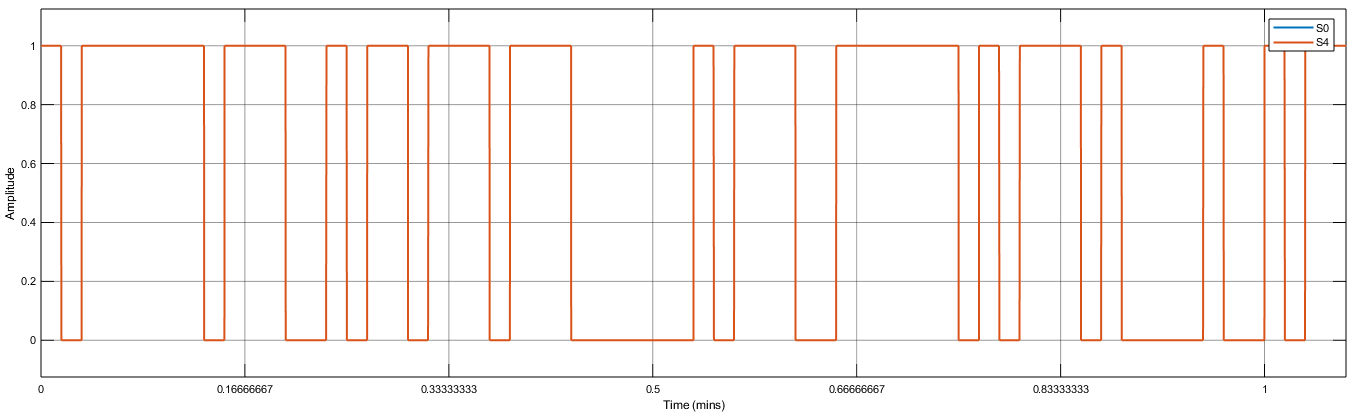
\includegraphics[width=.9\linewidth]{./sdf/eit_25828_hamming_channel_encoder_decoder/images/S0_S4.png}
	\vspace{-3mm}
	\caption{Comparison of S0 and S4 Signals (Original and Decoded Signals)}
	\label{fig:hammingEncoderDecoder_S0_S4}
	\vspace{-3mm}
\end{figure}

\vspace{-3mm}

\subsection*{BER Comparison}

\vspace{-1mm}

In this subsection we show the observed BER relations between the inputed error probability in the channel and the actual BER on the output of the channel (Figure \ref{fig:hammingEncoderDecoder_BER_input_output_channel}) and the relation between the inputed probability of error of the channel and the BER on the output of the Hamming Decoder (Figure \ref{fig:hammingEncoderDecoder_BER_input_output}) .

\begin{figure}[h!]
	\vspace{-4mm}
	\centering
	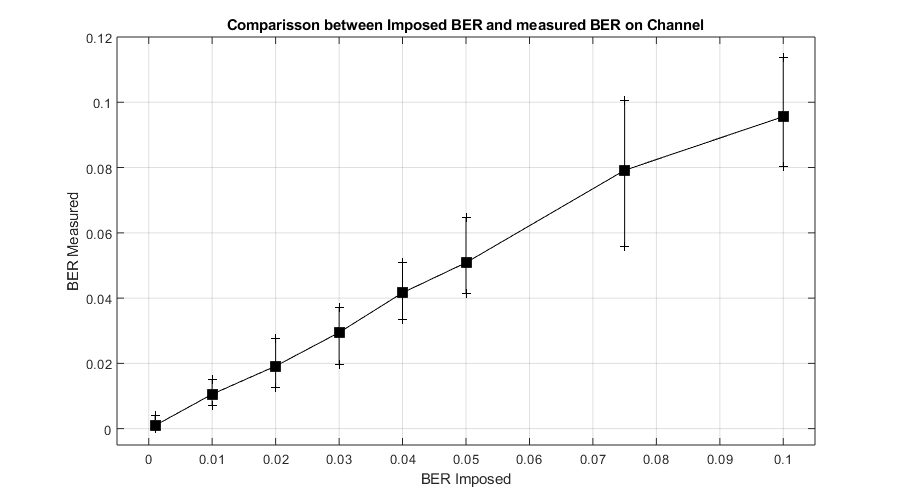
\includegraphics[width=.9\linewidth]{./sdf/eit_25828_hamming_channel_encoder_decoder/images/BER_1.png}
	\vspace{-5mm}
	\caption{Comparison between Imposed BER and measured BER on Channel}
	\label{fig:hammingEncoderDecoder_BER_input_output_channel}
\end{figure}

\begin{figure}[h!]
	\vspace{-9mm}
	\centering
	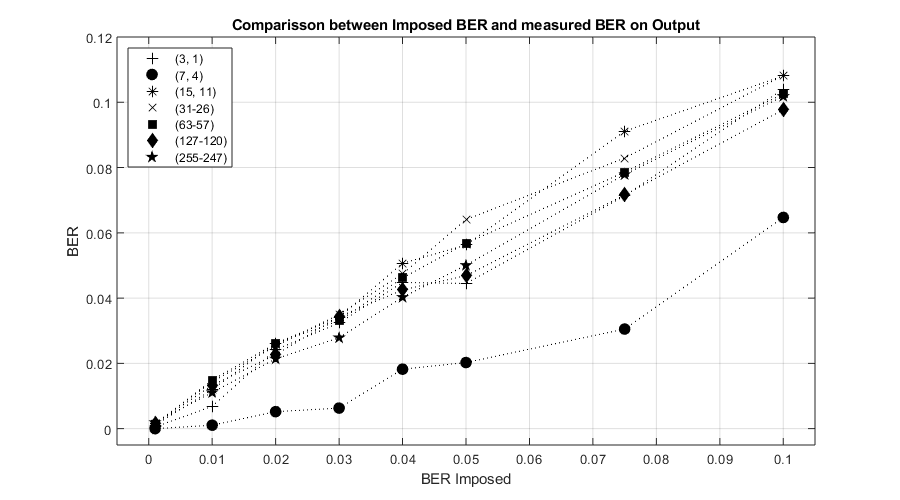
\includegraphics[width=.9\linewidth]{./sdf/eit_25828_hamming_channel_encoder_decoder/images/BER_2.png}
	\vspace{-5mm}
	\caption{Comparison between Imposed BER and measured BER on Output of Decoder}
	\label{fig:hammingEncoderDecoder_BER_input_output}
	\vspace{-30mm}
\end{figure}

\subsection*{Required files}
\label{Required files}

This project is composed by the header and source files described in following tables.

\begin{table}[H]
\centering
\begin{tabulary}{1.0\textwidth}{|p{7.5cm}|p{6.5cm}|p{1cm}|}
\hline
\multicolumn{3}{|c|}{ \textbf{Header Files} } \\
\hline
\textbf{File}                & \textbf{Comments} & \textbf{Status} \\ \hline
add\_20180620.h              &                   & \checkmark \\ \hline
binary\_source\_20180523.h   &                   & \checkmark \\ \hline
bit\_error\_rate\_20180424.h &                   & \checkmark \\ \hline
fork\_20180112.h             &                   & \checkmark \\ \hline
hamming\_coder\_20180608.h   &                   & \checkmark \\ \hline
hamming\_decoder\_20180608.h &                   & \checkmark \\ \hline
netxpto\_20180418.h          &                   & \checkmark \\ \hline
sink\_20180118.h             &                   & \checkmark \\ \hline

\end{tabulary}
\end{table}		
%
\begin{table}[H]
\centering
\begin{tabulary}{1.0\textwidth}{|p{9.5cm}|p{4.5cm}|p{1cm}|}
\hline
\multicolumn{3}{|c|}{ \textbf{Source Files} } \\
\hline
\textbf{File}              					  	   & \textbf{Comments} & \textbf{Status} \\ \hline
add\_20180620.cpp            				  	   &                   & \checkmark \\ \hline
binary\_source\_20180523.cpp   				  	   &                   & \checkmark \\ \hline
bit\_error\_rate\_20180424.cpp  				   &                   & \checkmark \\ \hline
fork\_20180112.cpp            				  	   &                   & \checkmark \\ \hline
hamming\_coder\_20180608.cpp   				  	   &                   & \checkmark \\ \hline
hamming\_decoder\_20180608.cpp 				  	   &                   & \checkmark \\ \hline
netxpto\_20180418.cpp         				  	   &                   & \checkmark \\ \hline
sink\_20180118.cpp            				  	   &                   & \checkmark \\ \hline
eit\_25828\_hamming\_channel\_encoder\_decoder.cpp &                   & \checkmark \\ \hline
\end{tabulary}
\end{table}		

\subsection*{System Input Parameters}

In order to successfully run this project it is required to set the following input parameters:

\begin{itemize}
	\item \textit{probalilityOfZero\_ErrorVector} $(p_{0})$ - Defines the probability for introducing errors (in order to simulate a non perfect channel). The probability of an error is $p_{1} = 1 - p_{0}$.
	\item \textit{hammingCode\_nBits} $n$ - Defines the Hamming Code coded word size.
	\item \textit{hammingCode\_kBits} $k$ - Defines the Hamming Code data size.
\end{itemize}

The $n$ and $k$, form the Hamming Code $(n, k)$, and the available combination of values for each of these variables can be viewed in the Hamming Encoder/Decoder in the Library Section.

\subsection*{Inputs}

This project doesn't take any input.

\subsection*{Outputs}

This project outputs the following signals:

\begin{itemize}
	\item \textbf{\textit{S0.sgn}} - The source binary signal.
	\item \textbf{\textit{S1.sgn}} - The encoded signal using the Hamming Code $(n, k)$.
	\item \textbf{\textit{S2.sgn}} - The noise signal.
	\item \textbf{\textit{S3.sgn}} - The resulting signal of adding the encoded signal $(S1.sgn)$ with the noise signal $(S2.sgn)$.
	\item \textbf{\textit{S4.sgn}} - The decoded signal using the Hamming Code $(n, k)$.
	\item \textbf{\textit{S5.sgn}} - The BER signal on the channel.
	\item \textbf{\textit{S6.sgn}} - The BER signal after decoding.
\end{itemize}

\subsection*{Open Issues}
\label{Open Issues}

The only issue found, at the time of the construction of these blocks, was not related to the developed blocks, but regarding another block, the Binary Source (\textit{binary\_source\_20180523.h}).

The mode \textit{Random} doesn't work as intended. The block requires the user to define a probability of Zero for the output of the block, but if the output buffer becomes full on the next time the block is called again to continue producing bits, the sequence is exactly the same (Figure \ref{fig:hammingEncoderDecoder_BinarySource_ERROR}). 

Observing the Figure below we can see a pattern that repeats itself over and over again instead of obtaining a completely random error vector.

\begin{figure}[h!]
	\centering
	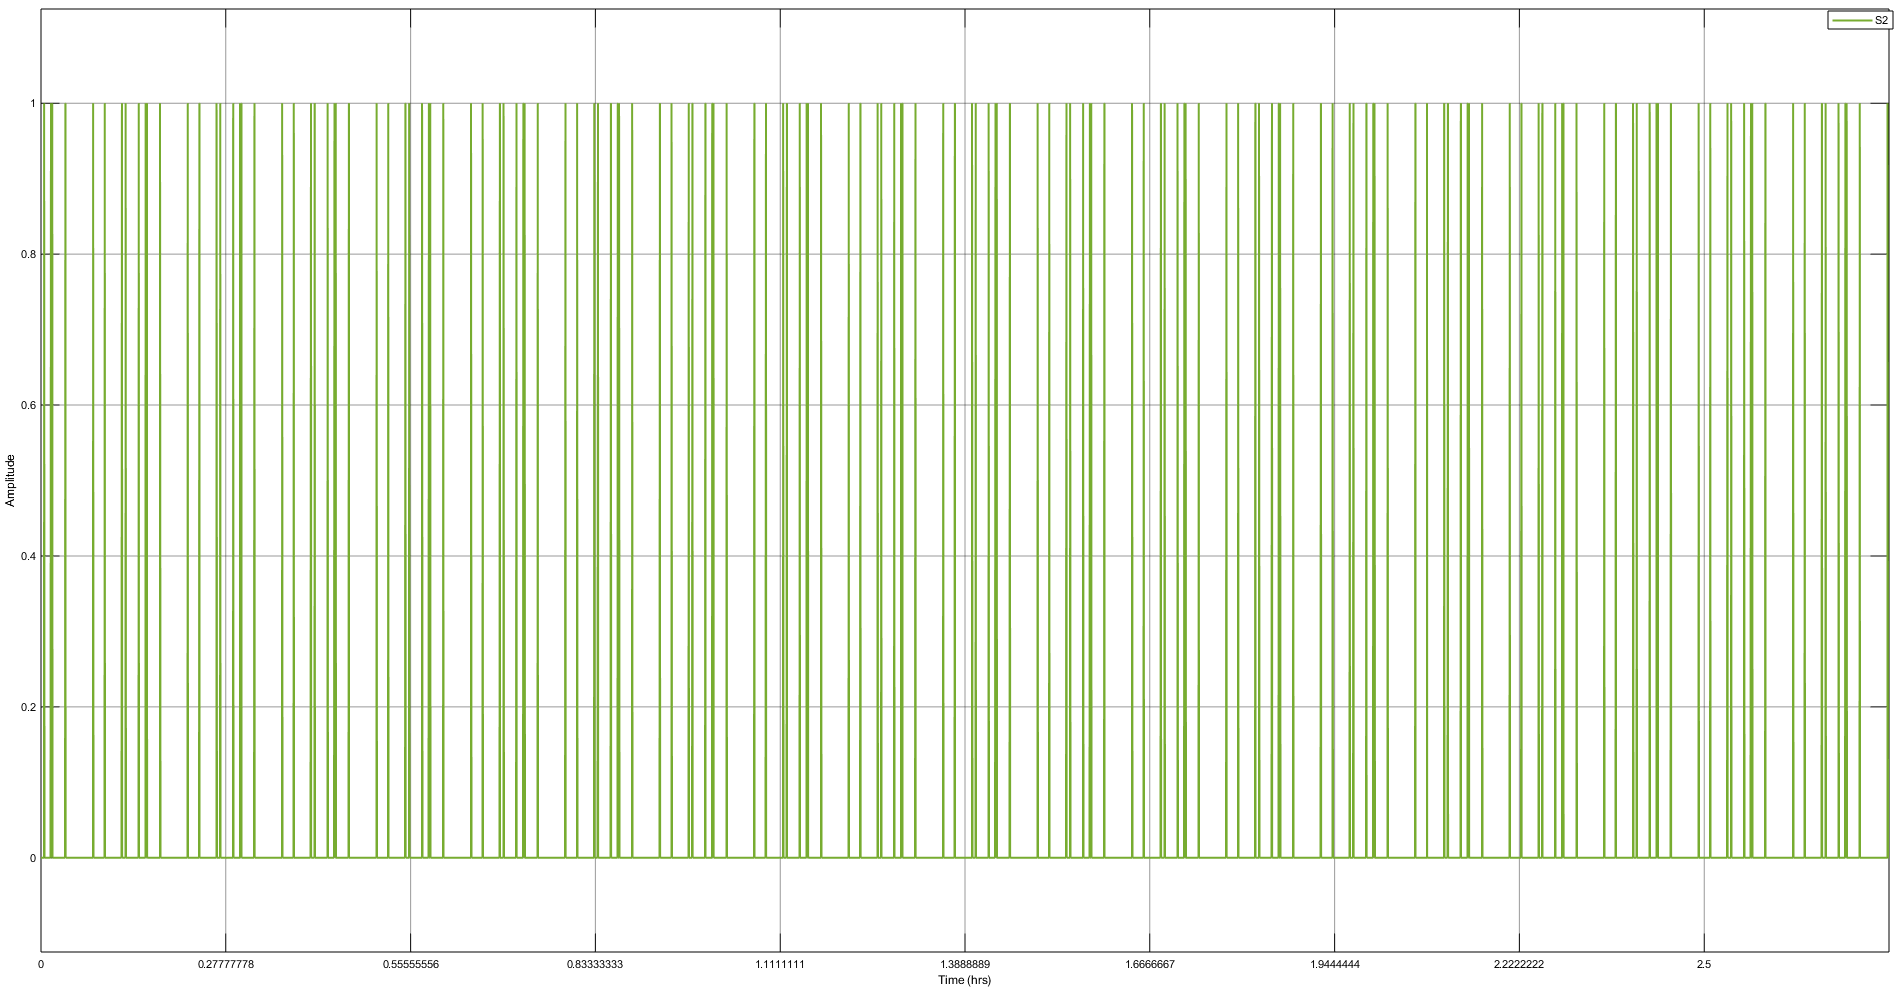
\includegraphics[width=.9\linewidth]{./sdf/eit_25828_hamming_channel_encoder_decoder/images/ERROR.png}
	\vspace{-3mm}
	\caption{Binary Source - Random mode - Observed Error}
	\label{fig:hammingEncoderDecoder_BinarySource_ERROR}
\end{figure}

\vspace{30mm}

This behavior needs to be resolved, not only to properly set this mode in the Binary Source, but also to improve the results of the developed blocks, since it is my belief that the curves observed in Figure \ref{fig:hammingEncoderDecoder_BER_input_output} would improved, reducing the BER observed on the output of the decoder for the same imposed BER.




% bibliographic references for the section ----------------------------
\clearpage
\printbibliography[heading=subbibliography]
\end{refsection}
\addcontentsline{toc}{subsection}{Bibliography}
\cleardoublepage
% --------------------------------------------------------------------- 